\chapter{I Was on Food Stamps... Now I Make \$100M/Year}

This School of Hard Knocks interview, curated by LazyingArt LLC through Video2Book, is arranged almost like a proof written backward. We are shown scale first and mechanism later: Beverly Hills spectacle, eight-figure personal income, a background of food stamps and government cheese, bankruptcy without surrender, the promise that everything could be rebuilt, and then, only afterward, the operating ideas that are supposed to make those outcomes intelligible. The lecture moves from display to distinction, from distinction to method, and from method to a broader philosophy of wealth.

\section{Cold Open and Formal Reset}

The episode does not begin with premises. It begins with a teaser splice. We hear fragments that belong to later parts of the conversation: the most money made in a year, the refusal of a broke mindset, the claim that everything could be rebuilt, the preference for buying businesses, and a brief turn toward faith. The structure matters. We are meant to feel the theorem before we are walked through the lemmas.

The first and most important separation arrives at once. The host asks for the biggest single-year number across companies, and then immediately asks, in effect, for the personal figure. The lecture therefore distinguishes company scale from the speaker's own one-year income:
\begin{align}
R_{\text{companies,max}} &\approx \$90\text{--}\$100\,\text{million}, \\
Y_{\text{personal}} &\approx \$25\,\text{million}.
\end{align}
This distinction should be preserved throughout. The transcript is conversational, but it is not sloppy on this point.

\begin{figure}[h]
\centering

\includegraphics[width=0.78\textwidth]{lecture_53_figure_02.png}
\caption{The interview's explicit visual evidence for the speaker's personal one-year money claim.}
\end{figure}

The visible numerical claim can then be reconstructed, cautiously, as
\begin{equation}
Y_{\text{personal}} \approx \$25\,\text{million}.
\end{equation}
The image itself carries only the number, not an accounting label, so the notation is interpretive rather than literally on screen.

Only after this teaser does the host rewind the tape and formally set the scene: Hidden Hills, Beverly Hills, a \(\$100\) million entrepreneur, a \(\$50\) million mansion, roughly ten companies, and a portfolio framed as doing more than \(\$100\) million a year. These host-side scale markers are part of the lecture's setup:
\begin{align}
V_{\text{house}} &\approx \$50\,\text{million}, \\
N_{\text{companies}} &\approx 10, \\
R_{\text{portfolio,current}} &> \$100\,\text{million}/\text{year}.
\end{align}
They tell us what sort of witness the lecture intends to put before us.

\subsection{Question \& Answer}

\paragraph{Question.} What exactly is being measured here: company revenue or personal income?

\paragraph{Answer.} Both appear, but not under the same sign. The larger figure belongs to company revenue across the speaker's businesses; the smaller visible figure belongs to what he says he made for himself. The interview's first task is therefore classificatory. Before we can learn anything from the numbers, we must know which balance sheet they live on.

\section{From Scale Back to Origin}

Once the formal interview begins, the lecture first establishes operating credibility. The speaker has lived in Beverly Hills for roughly four years, has been a business owner for most of his life, built and sold a tech-services business, built and sold a construction business, and now operates a supplement business while owning just under ten companies. This is not offered as a résumé for its own sake. It is there so that later advice arrives with a visible operating history behind it.

Then the direction reverses. The conversation moves from scale back to childhood: no rich parents, a mother pregnant at fourteen, the South, food stamps, government cheese, and the wish to get out. The lecture does not sentimentalize this material. It extracts from it a distinction:
\begin{equation}
\text{no money} \neq \text{broke mindset}.
\end{equation}
This equation is crude in form and precise in use. The speaker is willing to say that he had no money. He is unwilling to grant that his thinking was thereby determined. Later remarks about bankruptcy and rebuilding depend on exactly this distinction.

We should also notice the temporal order of ambition. The speaker does not say that as a child he clearly envisioned a hundred-million-dollar company. The more primitive fact comes first: he did not want to remain where he was. The desire for scale is initially directional rather than numerical. Only later does it condense into business size and income size.

\subsection{Question \& Answer}

\paragraph{Question.} What is the difference between having no money and having a broke mindset?

\paragraph{Answer.} In the lecture, having no money is a condition. A broke mindset is an internal limit accepted as final. One can suffer the first without ratifying the second. That is why food stamps, hardship, bankruptcy, and the repeated line ``I ain't never going back'' can all belong to one story without collapsing into fatalism.

\section{From Hours to Systems}

The next movement is the first explicitly portable doctrine. Asked for financial advice, the speaker does not begin with an asset class. He begins with a structural warning: do not keep trading dollars for hours as though that were the whole game. In its simplest form, labor income is
\begin{equation}
Y_{\text{labor}} = r_h H,
\end{equation}
where \(r_h\) is the hourly rate and \(H\) is the number of hours sold. The lecture's point is that \(H\) is finite. If we write that bound schematically as \(H \le H_{\max}\), then
\begin{equation}
Y_{\text{labor}} \le r_h H_{\max}.
\end{equation}
However high \(r_h\) may become, the structure itself has a ceiling.

The counter-idea is stated in the language of systems, passive income, and making money while one sleeps. We may write the intended condition as
\begin{equation}
Y_{\text{sleep}} > 0.
\end{equation}
This does not mean effortless wealth. It means that the machine one builds should continue to produce even when one's immediate labor has stopped for the night.

\subsection{Question \& Answer}

\paragraph{Question.} How do we stop trading time for money?

\paragraph{Answer.} The lecture does not tell us to despise work. It tells us not to stop at work. We begin, perhaps, with \(Y_{\text{labor}}\), but the task is to convert labor into a system, asset, or business that keeps producing when we are absent. That is what the speaker means by making money in one's sleep. The equation changes from pure presence to durable structure.

This transition is one of the lecture's most important hinges. Once we accept that the labor model is bounded, the next question is unavoidable: what should we build, buy, or enter now?

\section{Buy the Playbook}

Here the lecture narrows from general doctrine to action. Real estate is allowed as a respectable route, though the speaker notes that it often requires substantial capital. But the stronger answer is different: if one were starting today, one would buy businesses.

The key phrase is that the playbook already exists. In compressed form,
\begin{equation}
\text{existing business} \to \text{existing playbook} \to \text{faster path than starting from zero}.
\end{equation}
The host later pushes the point further by asking whether, if everything were lost tomorrow, it could all be made back. The answer is yes, and the reason offered is again acquisition: one can buy based on the business's own credit, use creative financing, and step into an already working machine.

When the host tentatively labels this ``the private equity model,'' the speaker corrects the scale. Not private equity in the institutional sense, he says, but leveraged buyouts. The lecture is not describing a Wall Street fund. It is describing a small- to medium-scale acquisition logic in which existing cash flow helps service acquisition debt.

\subsection{Question \& Answer}

\paragraph{Question.} Why buy a business instead of building one from scratch?

\paragraph{Answer.} Because a working business is condensed knowledge. Customers, operating rhythm, pricing, and proof of demand are already present. The lecture's point is not merely that buying is quicker. It is that buying allows us to inherit answers to questions that most founders spend years solving badly, if they solve them at all.

The lecture then sharpens into its most explicit arithmetic. The speaker names target businesses --- laundromats, pool companies, vending machines, other cash-flowing operations --- and gives a monthly spread example.

\paragraph{Worked Example.} Let
\begin{align}
CF_{\text{business}} &\approx \$20{,}000/\text{month}, \\
DS &\approx \$7{,}000\text{--}\$10{,}000/\text{month},
\end{align}
where \(CF_{\text{business}}\) is monthly cash flow and \(DS\) is monthly debt service. Define the retained spread by
\begin{equation}
S = CF_{\text{business}} - DS.
\end{equation}
The operative condition is simply
\begin{equation}
S > 0.
\end{equation}
That is the mathematical heart of the example. The business must throw off enough cash to service the acquisition debt and still remain positive.

The transcript then rounds the example toward a retained upside of about
\begin{equation}
S \approx \$10{,}000/\text{month}.
\end{equation}
Taken literally, the lower debt-service figure would leave a somewhat larger spread. The lecture's point, however, is not the last dollar of the estimate. It is the sign of the spread: the acquired business remains cash-flow positive after debt service.

We can therefore state the acquisition logic in short steps:
\begin{enumerate}
\item Find a business whose cash flow is already visible.
\item Use SBA \(7\)A financing or another creative structure to fund the purchase.
\item Service the debt from the business's operating cash flow.
\item Retain the positive spread \(S\).
\end{enumerate}

\begin{figure}[h]
\centering
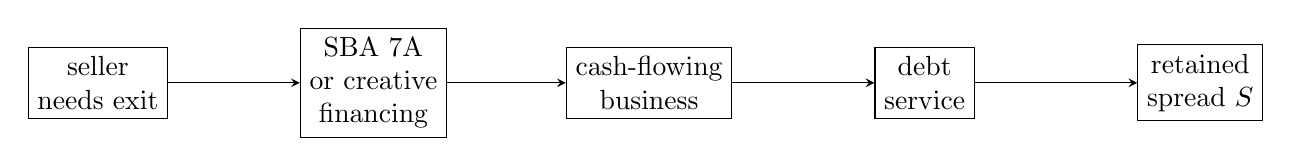
\begin{tikzpicture}[>=stealth]
\node[draw, rectangle, align=center] (a) at (0,0) {seller\\needs exit};
\node[draw, rectangle, align=center] (b) at (3.5,0) {SBA \(7\)A\\or creative\\financing};
\node[draw, rectangle, align=center] (c) at (7.0,0) {cash-flowing\\business};
\node[draw, rectangle, align=center] (d) at (10.5,0) {debt\\service};
\node[draw, rectangle, align=center] (e) at (14.0,0) {retained\\spread \(S\)};

\draw[->] (a) -- (b);
\draw[->] (b) -- (c);
\draw[->] (c) -- (d);
\draw[->] (d) -- (e);
\end{tikzpicture}
\caption{A compact reconstruction of the lecture's acquisition logic: exit pressure, financing, cash flow, debt service, and retained spread.}
\end{figure}

\section{The Gray Tsunami}

Having urged us to buy businesses, the lecture immediately asks the necessary next question: where do we find them? The answers descend from generality to method. There are listing portals, business brokers, and cold calls. The cold-call point is especially important. Some owners, the speaker says, would sell if someone simply asked them, because the desire to exit exists before the formal sales process begins.

Then the frame widens again. The host recasts the point as a transfer of wealth, and the speaker introduces the phrase ``gray tsunami.'' The content is demographic rather than mystical: many older owners need to leave their businesses, while many children do not want to inherit them. As a compact reconstruction,
\begin{equation}
N_{\text{sellers}} > N_{\text{buyers}}.
\end{equation}
This is not an on-screen statistic. It is a structural summary of the lecture's claim that the present market contains more aging-owner exits than prepared acquirers.

We should also preserve the reasons given for sale pressure: divorce, illness, fatigue, missing succession plans, children choosing other lives. These details keep the idea from sounding like abstract market timing. The lecture is arguing that acquisition becomes more plausible when personal exit pressure and demographic timing coincide.

At this point the chapter should resist a common simplification. The lesson is not merely ``buy a business.'' It is:
\begin{itemize}
\item an existing playbook is valuable,
\item seller pressure is real,
\item financing can be structured,
\item and the acquired cash flow must remain positive after debt service.
\end{itemize}
Only the conjunction of these conditions makes the recommendation as strong as the speaker intends.

\section{Interlude, Faith, and the Internal Driver}

A promotional interlude briefly interrupts the interview. It is easy to discard this as nonessential, but structurally it repeats one of the lecture's persistent ideas: blueprint matters, mentorship matters, proximity to people who have already done the thing matters. When the conversation resumes, however, it does so on a different register. The God question that had appeared in the teaser is now answered in full.

The speaker tells a childhood story: poverty, tears, doubt, a plea for God to show Himself, and then an unexpected encounter at work that becomes decisive. The lecture does not leave the story at the level of confession. It extracts from it a practical operator's rule:
\begin{equation}
\text{belief} \to \text{actions},\ \text{thought},\ \text{relationships}.
\end{equation}
That is the business use of the story. Belief is treated as a causal variable. It changes conduct, and conduct changes what kinds of relationships and opportunities become thinkable.

\subsection{Question \& Answer}

\paragraph{Question.} Why does faith matter practically in business rather than only spiritually?

\paragraph{Answer.} Because in the lecture belief is not decorative. It is generative. If we truly believe something, we act under that belief, interpret setbacks under that belief, and enter relationships under that belief. The point is not to smuggle theology into a spreadsheet. The point is to explain why interior conviction can have exterior economic effects.

The next question narrows again. College, the speaker says, did help, but only in a limited way: it gave him a programming skill and a programming job. It did not make him wealthy by itself. That prepares the lecture's next distinction between skill acquisition and market recognition.

\section{Skill, Marketing, and the Expansion of the Possible}

From college the lecture moves to business school and then to marketing. This order is important. First the speaker admits that education gave him a skill; then he says that formal business education misses something crucial. What it misses is not ``business'' in the abstract. It misses the fact that people may need what one has and still not know that one exists:
\begin{equation}
\text{people need you} \land \neg(\text{they know you}) \to \text{marketing problem}.
\end{equation}
Its positive form is
\begin{equation}
\text{need} \to \text{visibility} \to \text{growth}.
\end{equation}
The vivid instruction to get to the highest mountaintop and tell people who you are is a theory of exposure. One may have competence, product, and even genuine market need, and still fail if obscurity persists.

\subsection{Question \& Answer}

\paragraph{Question.} What does business school fail to teach once the product or skill already exists?

\paragraph{Answer.} In the lecture, the missing term is visibility. School may tell us how firms operate, but it does not sufficiently emphasize that unknown value remains economically inert. If the right people do not know we exist, then the bottleneck is not our internal knowledge. It is the market's ignorance of us.

Only after this does the lecture return to the environmental question that had also been teased earlier: has being in Los Angeles helped? The speaker then walks through Beverly Park, points out celebrity compounds and extreme car collections, and makes the real claim. Exposure changes the visible ceiling. Once certain scales of life and ownership become normal to the eye, they are difficult to erase from imagination:
\begin{equation}
\text{see larger ceiling} \to \text{cannot unsee possibility}.
\end{equation}
This is why the place-tour is not filler. It completes the lecture's final argument about vision.

The closing worldview follows directly. Wealthy people, in the speaker's description, do not primarily organize themselves around fixed ladders, preset salaries, and tightly pre-structured ceilings. They look for solvable problems and monetizable solutions:
\begin{equation}
\text{problem} \to \text{solution} \to \text{money}.
\end{equation}
The striking line that wealthy people ``don't need structure'' should therefore be read carefully. It does not mean they despise systems. It means they are less willing to confuse inherited structure with the outer boundary of possibility.

\section{Summary}

The lecture begins with spectacle and ends with method. First we are shown scale, then we separate company revenue from personal income, then we rewind to poverty and mindset, then move forward into the labor ceiling, the turn toward systems, the purchase of existing playbooks, the arithmetic of acquisition, and the demographic pressure of the gray tsunami. Only after those mechanisms are on the page does the lecture widen again to faith, skill, marketing, exposure, and the larger question of what one can imagine.

What remains is not a bag of slogans. It is a chain of distinctions:
\begin{align}
\text{no money} &\neq \text{broke mindset}, \\
Y_{\text{labor}} &\not\equiv Y_{\text{sleep}}, \\
\text{existing business} &\neq \text{blank page}, \\
\text{need} &\neq \text{visibility}.
\end{align}
The episode's deepest claim is that wealth is built not only by adding numbers, but by separating concepts that ordinary ambition often confuses. Once those separations are seen clearly, the field of action itself begins to widen.